\subsection{OpenStreetMap}
OpenStreetMap is a wiki page for maps and other geographical facts.People gather location data from a variety of sources such as recordings from GPS devices, from free satellite imagery or simply from knowing an area, and upload this data to OpenStreetMap. The uploaded data can be further modified, corrected and enriched by anyone who notices missing facts or errors.\\

\subsection{Steps to add to OpenStreetMap}
\begin{description}
\item[collecting Data] There are variety of ways of gathering data for OSM:
\begin{itemize}
\item Using GPS(Global Positioning Device) for tracking the paths to be mapped.
\item Having Local Knowledge of the area.
\item Using the imagery of the area to be mapped
\end{itemize}
\item[Uploading GPS data] The data we, collect in our GPS device is raw and for uploading it to OSM, following steps are to be followed:
\begin{itemize}
\item The raw data collected by us is in CSV(Comma-Seperated Values) and it need to be converted into GPX (GPS eXchange Format). It can easily be done by using the GPX convertor.
\item Once you have a GPX file containing a GPS trace, you should upload it to the site
\item Now download the area containing those traces into JOSM
\end{itemize}
\item[Create/Edit OSM data] Now edit the map of the area downloaded and make the editing according to the knowledge of the area or the data collected by GPS device.
\end{description}
\newpage
\subsection{Screenshot for Jalalabad mapping}
\begin{figure}[h]
\centering 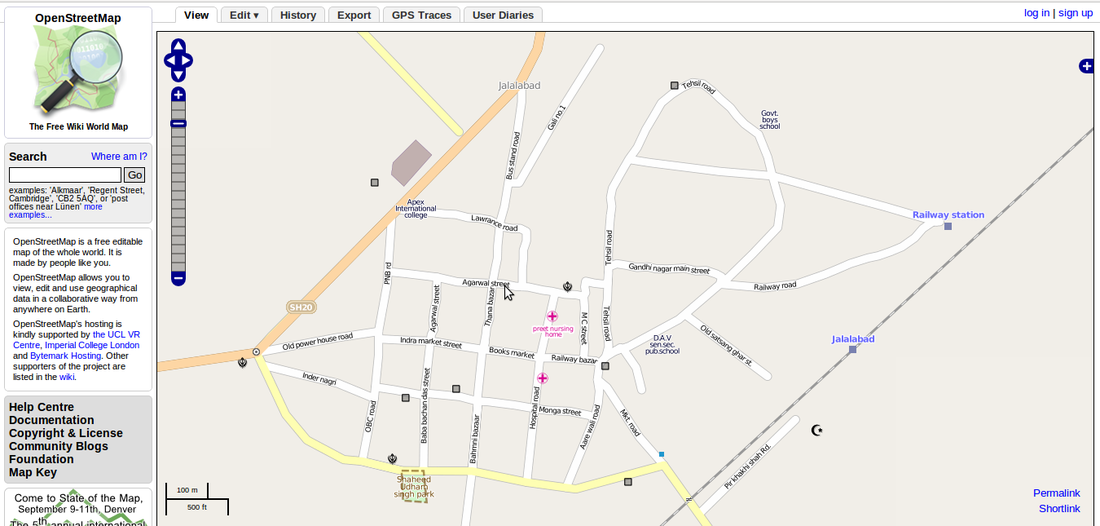
\includegraphics[scale=0.4]{ss1.png}
\caption{OSM map of jalalabad}
\end{figure}



 
